\documentclass[aspectratio=169,10pt]{beamer}

% ── Theme ────────────────────────────────────────────────────────────────────
\usetheme{Madrid}
\usecolortheme{whale}
\usefonttheme{professionalfonts}
\setbeamertemplate{navigation symbols}{}
\setbeamertemplate{caption}[numbered]

% ── Packages ─────────────────────────────────────────────────────────────────
\usepackage{amsmath,amssymb,amsfonts}
\usepackage{mathtools}
\usepackage{bm}
\usepackage{xcolor}
\usepackage{booktabs}
\usepackage{array}
\usepackage{tikz}
\usepackage{pgfplots}
\pgfplotsset{compat=1.18}
\usetikzlibrary{arrows.meta,calc,shapes.geometric,positioning}

% ── Colours ──────────────────────────────────────────────────────────────────
\definecolor{darkblue}{RGB}{26,58,92}
\definecolor{midblue}{RGB}{46,109,164}
\definecolor{lightblue}{RGB}{214,232,247}
\definecolor{gold}{RGB}{204,153,0}
\definecolor{darkred}{RGB}{160,30,30}
\definecolor{green2}{RGB}{0,120,60}

\setbeamercolor{title}{fg=white,bg=darkblue}
\setbeamercolor{frametitle}{fg=white,bg=darkblue}
\setbeamercolor{block title}{fg=white,bg=midblue}
\setbeamercolor{block body}{fg=black,bg=lightblue!40}
\setbeamercolor{block title alerted}{fg=white,bg=darkred}
\setbeamercolor{block body alerted}{fg=black,bg=red!8}
\setbeamercolor{block title example}{fg=white,bg=green2}
\setbeamercolor{block body example}{fg=black,bg=green2!10}
\setbeamercolor{palette primary}{bg=darkblue,fg=white}
\setbeamercolor{palette secondary}{bg=midblue,fg=white}
\setbeamercolor{palette tertiary}{bg=gold,fg=black}
\setbeamercolor{structure}{fg=darkblue}
\setbeamercolor{itemize item}{fg=midblue}
\setbeamercolor{itemize subitem}{fg=gold}
\setbeamercolor{enumerate item}{fg=midblue}

% ── Math macros ───────────────────────────────────────────────────────────────
\newcommand{\R}{\mathbb{R}}
\newcommand{\Hess}{\nabla^2}
\newcommand{\grad}{\nabla}
\newcommand{\norm}[1]{\left\|#1\right\|}
\newcommand{\lnorm}[2]{\left\|#1\right\|_{#2}}
\newcommand{\ip}[2]{\left\langle #1,\, #2 \right\rangle}
\newcommand{\Nx}{n(x)}
\DeclareMathOperator*{\argmin}{argmin}

% ── Footline info ─────────────────────────────────────────────────────────────
\institute[CS 435]{CS 435 --- Algorithms for Convex Optimization\\
                   Yale University, 2018}
\author[Vishnoi]{Nisheeth Vishnoi}
\date{April 12, 2018}

% ─────────────────────────────────────────────────────────────────────────────
\begin{document}

% ══════════════════════════════════════════════════════════════════════════════
\title[Newton's Method]{\textbf{Newton's Method}\\
  \large A Second-Order Optimization Algorithm}
\subtitle{Derivation $\cdot$ Convergence Analysis $\cdot$ Riemannian Perspective}

\begin{frame}[plain]
  \titlepage
\end{frame}

% ══════════════════════════════════════════════════════════════════════════════
\begin{frame}{Lecture Outline}
  \tableofcontents
\end{frame}

% ══════════════════════════════════════════════════════════════════════════════
\section{Newton-Raphson Method}

\begin{frame}{Newton-Raphson Method: Root Finding}
  \begin{columns}[T]
    \column{0.52\textwidth}
      \begin{block}{Problem Statement}
        Given $g:\R\to\R$, find $r\in\R$ such that $g(r)=0$.
      \end{block}
      \vspace{0.3em}
      \begin{block}{Geometric Idea}
        \begin{itemize}
          \item Start at $x_0$ near a root
          \item Draw the \textbf{tangent line} at $(x_0, g(x_0))$
          \item Let $x_1$ = intersection with the $x$-axis
          \item Repeat: each step brings us \emph{closer} to the root
        \end{itemize}
      \end{block}
      \vspace{0.3em}
      \begin{alertblock}{Update Rule}
        \[
          x_{k+1} \;:=\; x_k - \frac{g(x_k)}{g'(x_k)}, \qquad k \ge 0
        \]
        Requires: $g \in C^2$ (twice continuously differentiable)
      \end{alertblock}

    \column{0.44\textwidth}
      \begin{center}
      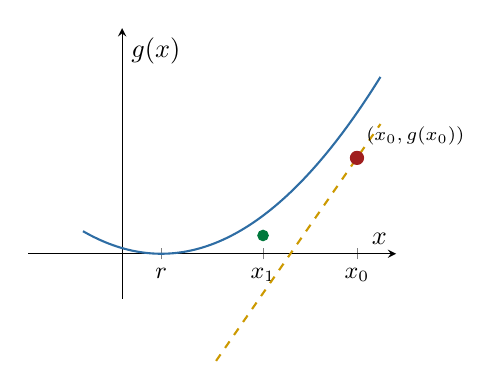
\begin{tikzpicture}[scale=0.95]
        \begin{axis}[
          width=6.5cm, height=5.2cm,
          axis lines=center,
          xlabel={$x$}, ylabel={$g(x)$},
          xmin=-1.2, xmax=3.5, ymin=-1, ymax=5,
          xtick={0.5,1.8,3.0},
          xticklabels={$r$,$x_1$,$x_0$},
          ytick=\empty,
          tick label style={font=\small},
          clip=false,
        ]
          \addplot[domain=-0.5:3.3, thick, midblue, samples=80]
            {0.5*(x-0.5)^2};
          % tangent at x0=3
          \addplot[domain=1.2:3.3, thick, gold, dashed]
            {2.5*(x-3)+2.125};
          \addplot[only marks, mark=*, mark size=2.5pt, darkred]
            coordinates {(3,2.125)};
          \addplot[only marks, mark=*, mark size=2pt, green2]
            coordinates {(1.8,0.405)};
          \node[font=\scriptsize,above right] at (axis cs:3,2.2) {$(x_0,g(x_0))$};
        \end{axis}
      \end{tikzpicture}
      \end{center}
      \vspace{-0.2em}
      \small Tangent at $x_0$ intersects $x$-axis at $x_1$, closer to root $r$.
  \end{columns}
\end{frame}

% ──────────────────────────────────────────────────────────────────────────────
\begin{frame}{Example: Computing $1/a$ Without Division}
  \begin{columns}[T]
    \column{0.5\textwidth}
      \begin{block}{Setup}
        Minimise $f(x)=ax-\log x$ over $x>0$.
        \[
          g(x) = f'(x) = a - \tfrac{1}{x}
          \;\Rightarrow\; r = \tfrac{1}{a}
        \]
      \end{block}
      \vspace{0.3em}
      \begin{block}{Newton Iteration}
        \[
          x_{k+1} = 2x_k - a\,x_k^2
        \]
        \textbf{No division required!} (only $+$ and $\times$)\\[0.3em]
        \emph{Historical note:} IBM used this trick in hardware.
      \end{block}

    \column{0.46\textwidth}
      \begin{exampleblock}{Convergence Analysis}
        Let $e_k := 1 - ax_k$.  Then:
        \[
          e_{k+1} = e_k^2
        \]
        \begin{itemize}
          \item $|e_0|<1$: \;\;$e_k\to 0$ \;\checkmark
          \item $|e_0|=1$: \;\;$e_k=1$, stuck
          \item $|e_0|>1$: \;\;$e_k\to\infty$ \;\;$\times$
        \end{itemize}
        In terms of $x_0$: converges iff $0 < x_0 < \tfrac{2}{a}$
      \end{exampleblock}
      \vspace{0.2em}
      \begin{alertblock}{Key Lesson}
        The \textbf{initial point} is critical for Newton's method!
      \end{alertblock}
  \end{columns}
\end{frame}

% ──────────────────────────────────────────────────────────────────────────────
\begin{frame}{Theorem 1: Quadratic Convergence}
  \begin{theorem}[Quadratic Convergence for Root Finding]
    Let $g:\R\to\R$ be $C^2$, $r$ a root, $x_0$ a starting point,
    $x_1 = x_0 - g(x_0)/g'(x_0)$.  Then:
    \[
      |r - x_1| \;\le\; M\,|r-x_0|^2,
      \qquad
      M = \sup_{\xi\in[r,x_0]} \left|\frac{g''(\xi)}{2\,g'(x_0)}\right|
    \]
  \end{theorem}

  \begin{columns}[T]
    \column{0.5\textwidth}
      \begin{block}{Proof Sketch}
        \begin{enumerate}
          \item Taylor-expand $g(r)=0$ at $x_0$ (MVT):
          \[
            0 = g(x_0) + (r-x_0)g'(x_0) + \tfrac{1}{2}(r-x_0)^2 g''(\xi)
          \]
          \item Use $g(x_0)=g'(x_0)(x_0-x_1)$
          \item Algebra gives $g'(x_0)(r-x_1) = \tfrac{1}{2}(r-x_0)^2 g''(\xi)$
          \item Divide by $|g'(x_0)|$ $\Rightarrow$ result
        \end{enumerate}
      \end{block}

    \column{0.46\textwidth}
      \begin{exampleblock}{Convergence Rate}
        If $M\le 1$ and $|x_0-r|<\tfrac{1}{2}$:
        \[
          |x_k - r| \;\le\; |x_0-r|^{2^k} \;\le\; 2^{-2^k}
        \]
        \vspace{0.2em}
        \textbf{To reach error $\varepsilon$:}
        \[
          k \;\approx\; \log\log\frac{1}{\varepsilon} \text{ steps}
        \]
        \emph{Doubly exponential} speed!\\[0.3em]
        Compare: gradient descent needs $O(1/\varepsilon)$.
      \end{exampleblock}
  \end{columns}
\end{frame}

% ──────────────────────────────────────────────────────────────────────────────
\begin{frame}{Extension to Multivariate Functions}
  \begin{columns}[T]
    \column{0.48\textwidth}
      \begin{block}{Setting}
        Find $x\in\R^n$ satisfying the system
        $g_1(x)=\cdots=g_n(x)=0$,
        i.e.\ $g:\R^n\to\R^n$, $g(x)=\mathbf{0}$.
      \end{block}
      \vspace{0.4em}
      \begin{block}{Jacobian Replaces Derivative}
        The Jacobian $J_g(x_0)\in\R^{n\times n}$:
        \[
          g(x) = g(x_0) + J_g(x_0)(x-x_0) + o(\norm{x-x_0}^2)
        \]
        \[
          \bigl[J_g(x_0)\bigr]_{ij} = \frac{\partial g_i}{\partial x_j}(x_0)
        \]
      \end{block}

    \column{0.48\textwidth}
      \begin{alertblock}{Multivariate Update Rule}
        \[
          x_{k+1} := x_k - J_g(x_k)^{-1}\,g(x_k), \quad k\ge 0
        \]
        Division $\to$ \textbf{matrix inversion}
      \end{alertblock}
      \vspace{0.4em}
      \begin{exampleblock}{Convergence}
        Local quadratic convergence still holds.
        The constant $M$ now involves:
        \begin{itemize}
          \item Upper bound on Lipschitz const.\ of $J_g$
          \item Lower bound: $1/\norm{J_g(x)^{-1}}$
        \end{itemize}
      \end{exampleblock}
  \end{columns}
\end{frame}

% ══════════════════════════════════════════════════════════════════════════════
\section{Newton's Method for Optimization}

\begin{frame}{From Root-Finding to Optimization}
  \begin{columns}[T]
    \column{0.48\textwidth}
      \begin{block}{Key Bridge}
        For smooth convex $f:\R^n\to\R$:
        \[
          x^* = \argmin_{x\in\R^n} f(x)
          \;\Longleftrightarrow\;
          \grad f(x^*) = \mathbf{0}
        \]
        Apply Newton's method to $g:=\grad f$!
      \end{block}
      \vspace{0.3em}
      \begin{block}{Newton Step \& Update}
        Since $J_{\grad f}(x) = \Hess f(x)$:
        \[
          \boxed{x_{k+1} := x_k - \bigl(\Hess f(x_k)\bigr)^{-1}\!\grad f(x_k)}
        \]
        Define the \textbf{Newton step} at $x$:
        \[
          n(x) := -\bigl(\Hess f(x)\bigr)^{-1}\!\grad f(x)
        \]
        So: $x_{k+1} = x_k + n(x_k)$
      \end{block}

    \column{0.48\textwidth}
      \begin{exampleblock}{Second-Order Interpretation}
        Minimise the local \textbf{quadratic approximation}:
        \[
          \tilde{f}(x) = f(x_0) + \ip{x-x_0}{\grad f(x_0)}
                        + \tfrac{1}{2}(x-x_0)^\top\!\Hess f(x_0)(x-x_0)
        \]
        Setting $\grad\tilde{f}(x)=0$ yields \emph{exactly} the Newton step!
        \vspace{0.3em}

        $\Rightarrow$ Newton's method = minimise a fresh quadratic at each step.
      \end{exampleblock}
      \vspace{0.3em}
      \begin{alertblock}{Computational Cost / Iteration}
        Solve $\Hess f(x_k)\,d = \grad f(x_k)$:
        \begin{itemize}
          \item General: $O(n^3)$ (Gaussian elimination)
          \item Structured (SDD, Laplacian): $\tilde{O}(m)$
        \end{itemize}
      \end{alertblock}
  \end{columns}
\end{frame}

% ──────────────────────────────────────────────────────────────────────────────
\begin{frame}{Example: Logarithmic Barrier \& Analytic Center}
  \begin{columns}[T]
    \column{0.5\textwidth}
      \begin{block}{Polytope \& Logarithmic Barrier}
        $P = \{x\in\R^n : \ip{a_i}{x}\le b_i,\; i=1,\ldots,m\}$
        \[
          F(x) = -\sum_{i=1}^{m}\log\bigl(b_i - a_i^\top x\bigr)
        \]
        Each term $\to+\infty$ as $x\to$ the $i$-th face.
      \end{block}
      \vspace{0.3em}
      \begin{block}{Gradient \& Hessian}
        With $s_i(x):=b_i-a_i^\top x$ (slack):
        \[
          \grad F(x) = \sum_{i=1}^{m}\frac{a_i}{s_i(x)}
        \]
        \[
          \Hess F(x) = \sum_{i=1}^{m}\frac{a_ia_i^\top}{s_i(x)^2}
        \]
      \end{block}

    \column{0.46\textwidth}
      \begin{exampleblock}{Analytic Center}
        The unique $x^*$ with $\grad F(x^*)=\mathbf{0}$ is called the
        \textbf{analytic center} of $P$.

        \vspace{0.2em}
        Physical view: equilibrium of $m$ repulsive forces.

        \vspace{0.2em}
        \textbf{Applications:}
        \begin{itemize}
          \item Assessing volume of $P$
          \item \textbf{Polynomial-time LP} (Renegar 1988)
        \end{itemize}
      \end{exampleblock}
      \vspace{0.3em}
      \begin{alertblock}{Complexity}
        $\grad F$: $O(nm)$;\quad $\Hess F$: $O(n^2 m)$\\
        Sparse $a_i$: both reduce to $O(m)$\\
        Graph Laplacian structure: $\tilde{O}(m)$ [Spielman--Teng]
      \end{alertblock}
  \end{columns}
\end{frame}

% ══════════════════════════════════════════════════════════════════════════════
\section{Convergence Analysis: Euclidean Norm}

\begin{frame}{Theorem 2: Quadratic Convergence (Euclidean Norm)}
  \begin{theorem}[Quadratic Convergence w.r.t.\ Euclidean Norm]
    Let $f:\R^n\to\R$, $x^*$ its minimizer, $x_0$ any starting point,
    $x_1:=x_0+n(x_0)$.
    If condition $\mathbf{NE}(M)$ holds, then
    \[
      \norm{x_1-x^*}_2 \;\le\; M\,\norm{x_0-x^*}_2^2
    \]
  \end{theorem}

  \begin{columns}[T]
    \column{0.5\textwidth}
      \begin{block}{Condition NE (Newton-Euclidean)}
        $\exists$ ball $B(x^*,R)\ni x_0$ and constants $h,L>0$
        with $M\ge\frac{L}{2h}$ such that:
        \begin{enumerate}
          \item $\norm{H(x)^{-1}}\le\frac{1}{h}$
                for all $x\in B(x^*,R)$
                \hfill(large $h$ $\Rightarrow$ large Hessian)
          \item $\norm{H(x)-H(y)}\le L\norm{x-y}_2$
                for all $x,y\in B(x^*,R)$
                \hfill(Hessian is $L$-Lipschitz)
        \end{enumerate}
      \end{block}

    \column{0.46\textwidth}
      \begin{block}{Proof Strategy}
        Using the Fundamental Theorem of Calculus:
        \[
          x_1-x^* = H(x_0)^{-1}\!\int_0^1\!\!
            \bigl(H(x_0\!+\!t\delta)-H(x_0)\bigr)\delta\,dt
        \]
        where $\delta:=x^*-x_0$.  Then:
        \[
          \norm{x_1-x^*}_2
          \le \frac{L\norm{H(x_0)^{-1}}}{2}\norm{x^*-x_0}_2^2
        \]
        Take $M = \frac{L\norm{H(x_0)^{-1}}}{2} \le \frac{L}{2h}$.
      \end{block}
  \end{columns}
\end{frame}

% ──────────────────────────────────────────────────────────────────────────────
\begin{frame}{Limitations: Why Euclidean Norm Fails}
  \begin{columns}[T]
    \column{0.5\textwidth}
      \begin{alertblock}{Failure Example}
        Polytope $P=[-K_1,K_1]\times[-1/K_2,1/K_2]\subseteq\R^2$,
        $K_1, K_2\gg 1$ (very elongated).
        \vspace{0.2em}
        \begin{itemize}
          \item At $x^*=(0,0)$: $h \le 2/K_1^2$ (tiny!)
          \item Lipschitz constant: $L \approx K_2^2$ (huge!)
          \item $M = L/(2h) = \Omega(K_1^2 K_2^2)$
        \end{itemize}
        \vspace{0.2em}
        Theorem 2 gives \textbf{no useful bound}, yet\\
        Newton's method converges rapidly in practice!
      \end{alertblock}

    \column{0.46\textwidth}
      \begin{block}{Affine Invariance of Newton's Method}
        Under any affine map $\varphi(x)=Ax+b$:
        \begin{itemize}
          \item Newton's \emph{trajectory is identical}
                in both $x$- and $y$-coordinates
          \item Gradient descent \textbf{does not} share this property
        \end{itemize}
        \vspace{0.3em}
        \textbf{Problem with Theorem 2:}
        $h$ and $L$ change under reparametrisation
        $\Rightarrow$ the bound is \emph{not affinely invariant}.
      \end{block}
      \vspace{0.3em}
      \begin{exampleblock}{Solution}
        Replace the Euclidean norm with the\\
        \textbf{local norm} induced by the Hessian.
      \end{exampleblock}
  \end{columns}
\end{frame}

% ══════════════════════════════════════════════════════════════════════════════
\section{Riemannian Manifold View}

\begin{frame}{Newton's Method as Gradient Descent on a Riemannian Manifold}
  \begin{columns}[T]
    \column{0.5\textwidth}
      \begin{block}{Motivating Example}
        Minimise $f(x_1,x_2)=x_1^2+Kx_2^2$, $K\gg 1$.
        \vspace{0.2em}
        \begin{itemize}
          \item Gradient descent with fixed $\eta$: overshoots ($\eta\approx 1/K$ needed)
          \item Use instead the \emph{Hessian norm}:
                $\norm{(u_1,u_2)}_\circ = \sqrt{u_1^2+Ku_2^2}$
          \item Steepest descent in $\norm{\cdot}_\circ$:
                $u_\text{opt} \propto -x$, points \emph{directly to $x^*=0$}
          \item For $\eta=1$: one step finds the exact minimum!
        \end{itemize}
      \end{block}

    \column{0.46\textwidth}
      \begin{block}{Local Inner Product \& Local Norm}
        For strictly convex $f$ with $H(x)=\Hess f(x)$:
        \[
          \ip{u}{v}_x := u^\top H(x)\,v
        \]
        \[
          \lnorm{u}{x} := \sqrt{u^\top H(x)\,u}
        \]
        These define a \textbf{Riemannian metric} on $\R^n$,
        varying smoothly with $x$.\\[0.3em]
        $\Rightarrow$ a \textbf{Hessian manifold}.
      \end{block}
      \begin{exampleblock}{Newton's Flow}
        Steepest descent w.r.t.\ $\lnorm{\cdot}{x}$:
        \[
          u_\text{opt} \propto -H(x)^{-1}\grad f(x) = n(x)
        \]
        Continuous limit:
        $\dfrac{dx}{dt} = -\bigl(\Hess f(x)\bigr)^{-1}\grad f(x)$
      \end{exampleblock}
  \end{columns}
\end{frame}

% ══════════════════════════════════════════════════════════════════════════════
\section{Affinely Invariant Analysis}

\begin{frame}{Theorem 4: Convergence in the Local Norm}
  \begin{block}{Potential Function (affinely invariant)}
    \[
      \lambda(x) := \lnorm{n(x)}{x}
               = \sqrt{\grad f(x)^\top H(x)^{-1}\grad f(x)}
    \]
    \emph{Interpretation:} $\tfrac{1}{2}\lambda(x)^2$
    = gap between $f(x)$ and minimum of its local quadratic approximation.
  \end{block}

  \begin{theorem}[Quadratic Convergence w.r.t.\ Local Norm]
    Let $f$ satisfy condition \textbf{NL}, $x_0\in\R^n$, $x_1:=x_0+n(x_0)$.
    \[
      \lambda(x_0) < \tfrac{1}{6}
      \;\Longrightarrow\;
      \lambda(x_1) \;\le\; 3\,\lambda(x_0)^2
    \]
  \end{theorem}

  \begin{columns}[T]
    \column{0.5\textwidth}
      \begin{block}{Condition NL (Newton-Local) --- affinely invariant}
        For all $x,y$ with $\lnorm{y-x}{x}=\delta<1$:
        \[
          (1-3\delta)H(x) \preceq H(y) \preceq (1+3\delta)H(x)
        \]
        Hessian changes proportionally to itself
        under one ``local unit'' of displacement.
      \end{block}

    \column{0.46\textwidth}
      \begin{exampleblock}{Proof Key Steps}
        \begin{enumerate}
          \item \textbf{Lemma 6} (low distortion):
                $\lnorm{y-x}{x}\le\tfrac{1}{6}$
                $\Rightarrow$ $\tfrac{1}{2}\lnorm{\cdot}{x}\le\lnorm{\cdot}{y}\le 2\lnorm{\cdot}{x}$
          \item Write $\grad f(x_1)=M(x_0)H(x_0)^{-1}\grad f(x_0)$ via FTC
          \item NL $+$ Fact 1 (PSD ordering):
                $\lnorm{H^{-1/2}MH^{-1/2}}{}\le\tfrac{3}{2}\lambda(x_0)$
          \item Combine $\Rightarrow$ Theorem 4
        \end{enumerate}
      \end{exampleblock}
  \end{columns}
\end{frame}

% ──────────────────────────────────────────────────────────────────────────────
\begin{frame}{Comparison of Convergence Analyses}
  \begin{center}
  \renewcommand{\arraystretch}{1.4}
  \begin{tabular}{lll}
    \toprule
    \textbf{Property} & \textbf{Theorem 2 (Euclidean)} & \textbf{Theorem 4 (Local Norm)} \\
    \midrule
    Progress measure
      & $\norm{x_1-x^*}_2 \le M\norm{x_0-x^*}_2^2$
      & $\lambda(x_1)\le 3\lambda(x_0)^2$ \\[2pt]
    Condition
      & NE: ball, constants $h,L$
      & NL: local Lipschitz on $H$ \\[2pt]
    Affinely invariant
      & \textcolor{darkred}{\textbf{No}} — $h,L$ change with coords
      & \textcolor{green2}{\textbf{Yes}} — all quantities invariant \\[2pt]
    Log-barrier failure
      & \textcolor{darkred}{\textbf{Yes}} — $M=\Omega(K_1^2K_2^2)$
      & \textcolor{green2}{\textbf{No}} — bounded for any $P$ \\[2pt]
    Proof tool
      & Lipschitz $H$ + operator norm
      & FTC + PSD ordering + Lemma 6 \\
    \bottomrule
  \end{tabular}
  \end{center}

  \vspace{0.8em}
  \begin{alertblock}{The Right Choice of Norm Matters}
    The Euclidean norm is a poor fit for Newton's method, which is
    intrinsically coordinate-free. The local (Hessian) norm restores
    affine invariance and gives a clean, universally applicable bound.
  \end{alertblock}
\end{frame}

% ══════════════════════════════════════════════════════════════════════════════
\section{Summary}

\begin{frame}{Key Takeaways}
  \begin{enumerate}\setlength\itemsep{0.55em}
    \item \textbf{Doubly-exponential convergence.}
          Near a root, $k\approx\log\log(1/\varepsilon)$ iterations suffice ---
          vastly better than first-order methods.

    \item \textbf{Second-order method.}
          Each step minimises the local quadratic approximation of $f$.
          One step is exact for strictly convex quadratics.

    \item \textbf{Cost--benefit trade-off.}
          Requires solving an $n{\times}n$ linear system per step
          ($O(n^3)$ general; $\tilde{O}(m)$ for Laplacians).

    \item \textbf{Affine invariance.}
          Newton's trajectory is coordinate-free.
          The local norm captures this correctly; the Euclidean norm does not.

    \item \textbf{Connection to interior-point methods.}
          Logarithmic barrier $+$ Newton's method yields a
          polynomial-time LP algorithm (Renegar 1988).
          Condition NL $\approx$ \emph{self-concordance}
          (Nesterov--Nemirovskii 1994).
  \end{enumerate}
\end{frame}

% ══════════════════════════════════════════════════════════════════════════════
\begin{frame}[allowframebreaks]{References}
  \begin{thebibliography}{5}
    \bibitem{Galntai2000}
      A.~Galntai.
      \newblock The theory of Newton's method.
      \newblock \emph{J. Comput. Appl. Math.}, 124(1):25--44, 2000.

    \bibitem{NesterovNemirovskii1994}
      Y.~Nesterov and A.~Nemirovskii.
      \newblock \emph{Interior-Point Polynomial Algorithms in Convex Programming}.
      \newblock SIAM, 1994.

    \bibitem{Raphson1690}
      J.~Raphson.
      \newblock \emph{Analysis aequationum universalis}.
      \newblock London, 1690.

    \bibitem{Renegar1988}
      J.~Renegar.
      \newblock A polynomial-time algorithm, based on Newton's method,
                for linear programming.
      \newblock \emph{Math. Program.}, 40(1--3):59--93, 1988.

    \bibitem{SpielmanTeng2004}
      D.~A.~Spielman and S.-H.~Teng.
      \newblock Nearly-linear time algorithms for graph partitioning,
                graph sparsification, and solving linear systems.
      \newblock In \emph{STOC 2004}, pages 81--90, 2004.
  \end{thebibliography}
\end{frame}

\end{document}
